\documentclass{article}
\usepackage{natbib}
\usepackage{amsmath}
\usepackage{tabularx}
\usepackage{graphicx}
\graphicspath{ {./images/} } 

\title{Happywhale - Whale and Dolphin Identification}
\author{Matthew Harding}
\date{April 2024}

\begin{document}

\maketitle

\section{Abstract}
This project explores the problem of classifiying images of dolphins and whales to identify indivduals. This work 
is based on the \emph{Happywhale - Whale and Dolphin Identification} Kaggle competition \cite{kaggle_comp}.

Data for this competition contains over 50,000 images of over 15,000 unique individual marine mammals from 30 different species collected from 28 different research organizations. 
Individuals have been manually identified and given an individual\_id by marine researchers.

The Kaggle competion had the additional complexity of requiring the ability to classify individuals not included in the training dataset. It was decided to ommit this requirement due to time limitations. The Kaggle competion also measured model performance via Mean Average Precision @ 5 but for this task it was replaced with Accuracy.

\section{Training Data}

\begin{figure}[!htb]
    \centering
    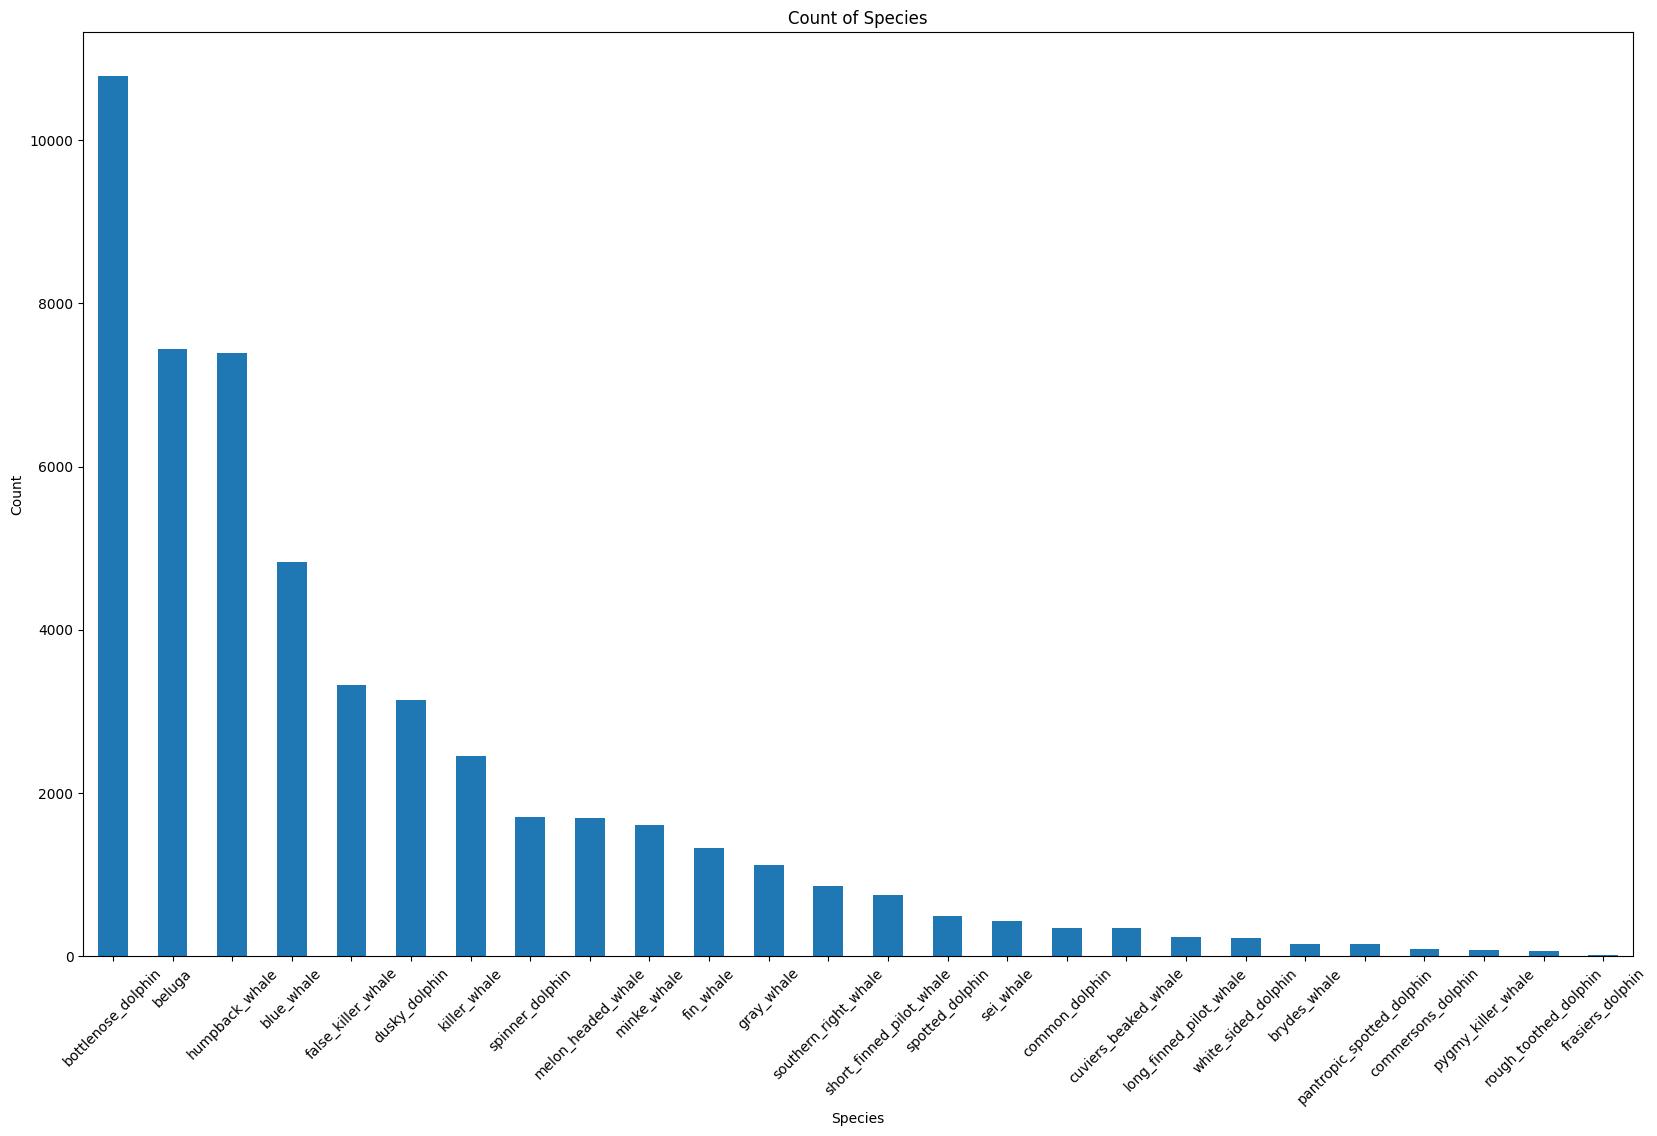
\includegraphics[width=0.8\textwidth]{species_histogram.png}
    \caption{Number of training images per species}
    \label{fig:species_count_histogram}
\end{figure}

\begin{figure}[!htb]
    \centering
    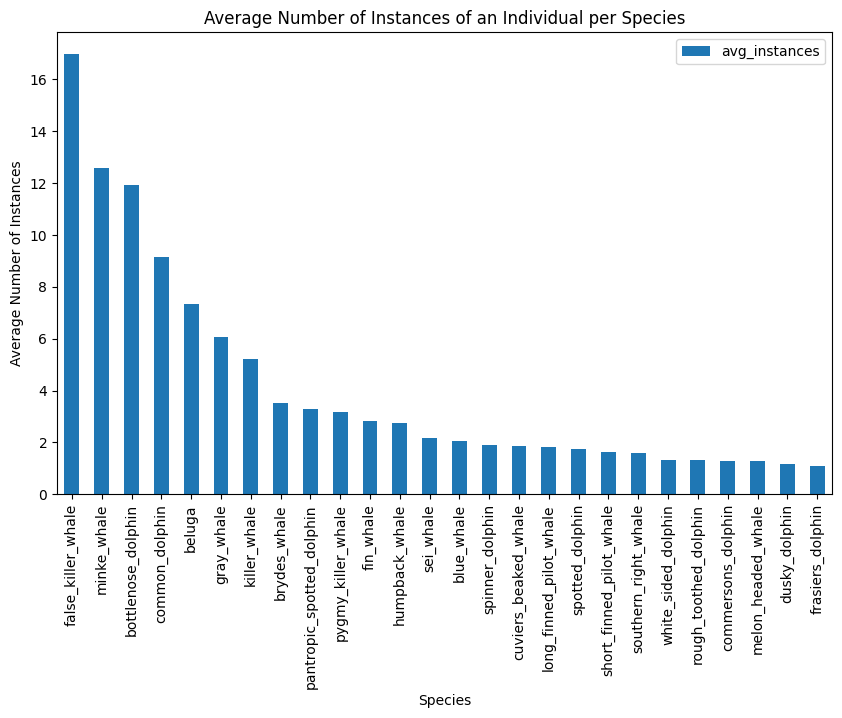
\includegraphics[width=0.8\textwidth]{mean_individuals_histogram.png}
    \caption{Mean count of images per individual by species}
    \label{fig:individual_mean_count_histogram}
\end{figure}

Looking at the histogram of species Figure \ref{fig:species_count_histogram}, there is a clear inbalance in the number of images per species with the vast majority
of labelled images being for bottlenose dolphins, beluga whales, humpback whales and blue whales. For some species the number of examples it so low it will be difficult to gain a high level of accuracy.

Figure \ref{fig:individual_mean_count_histogram} shows the mean count of images per indivdual by species where we see another imbalance with some species on average containing a large number of images per indivudal whilst others only contain one or two images per individual.


\section{Image Preprocessing}

\begin{figure}
    \centering
    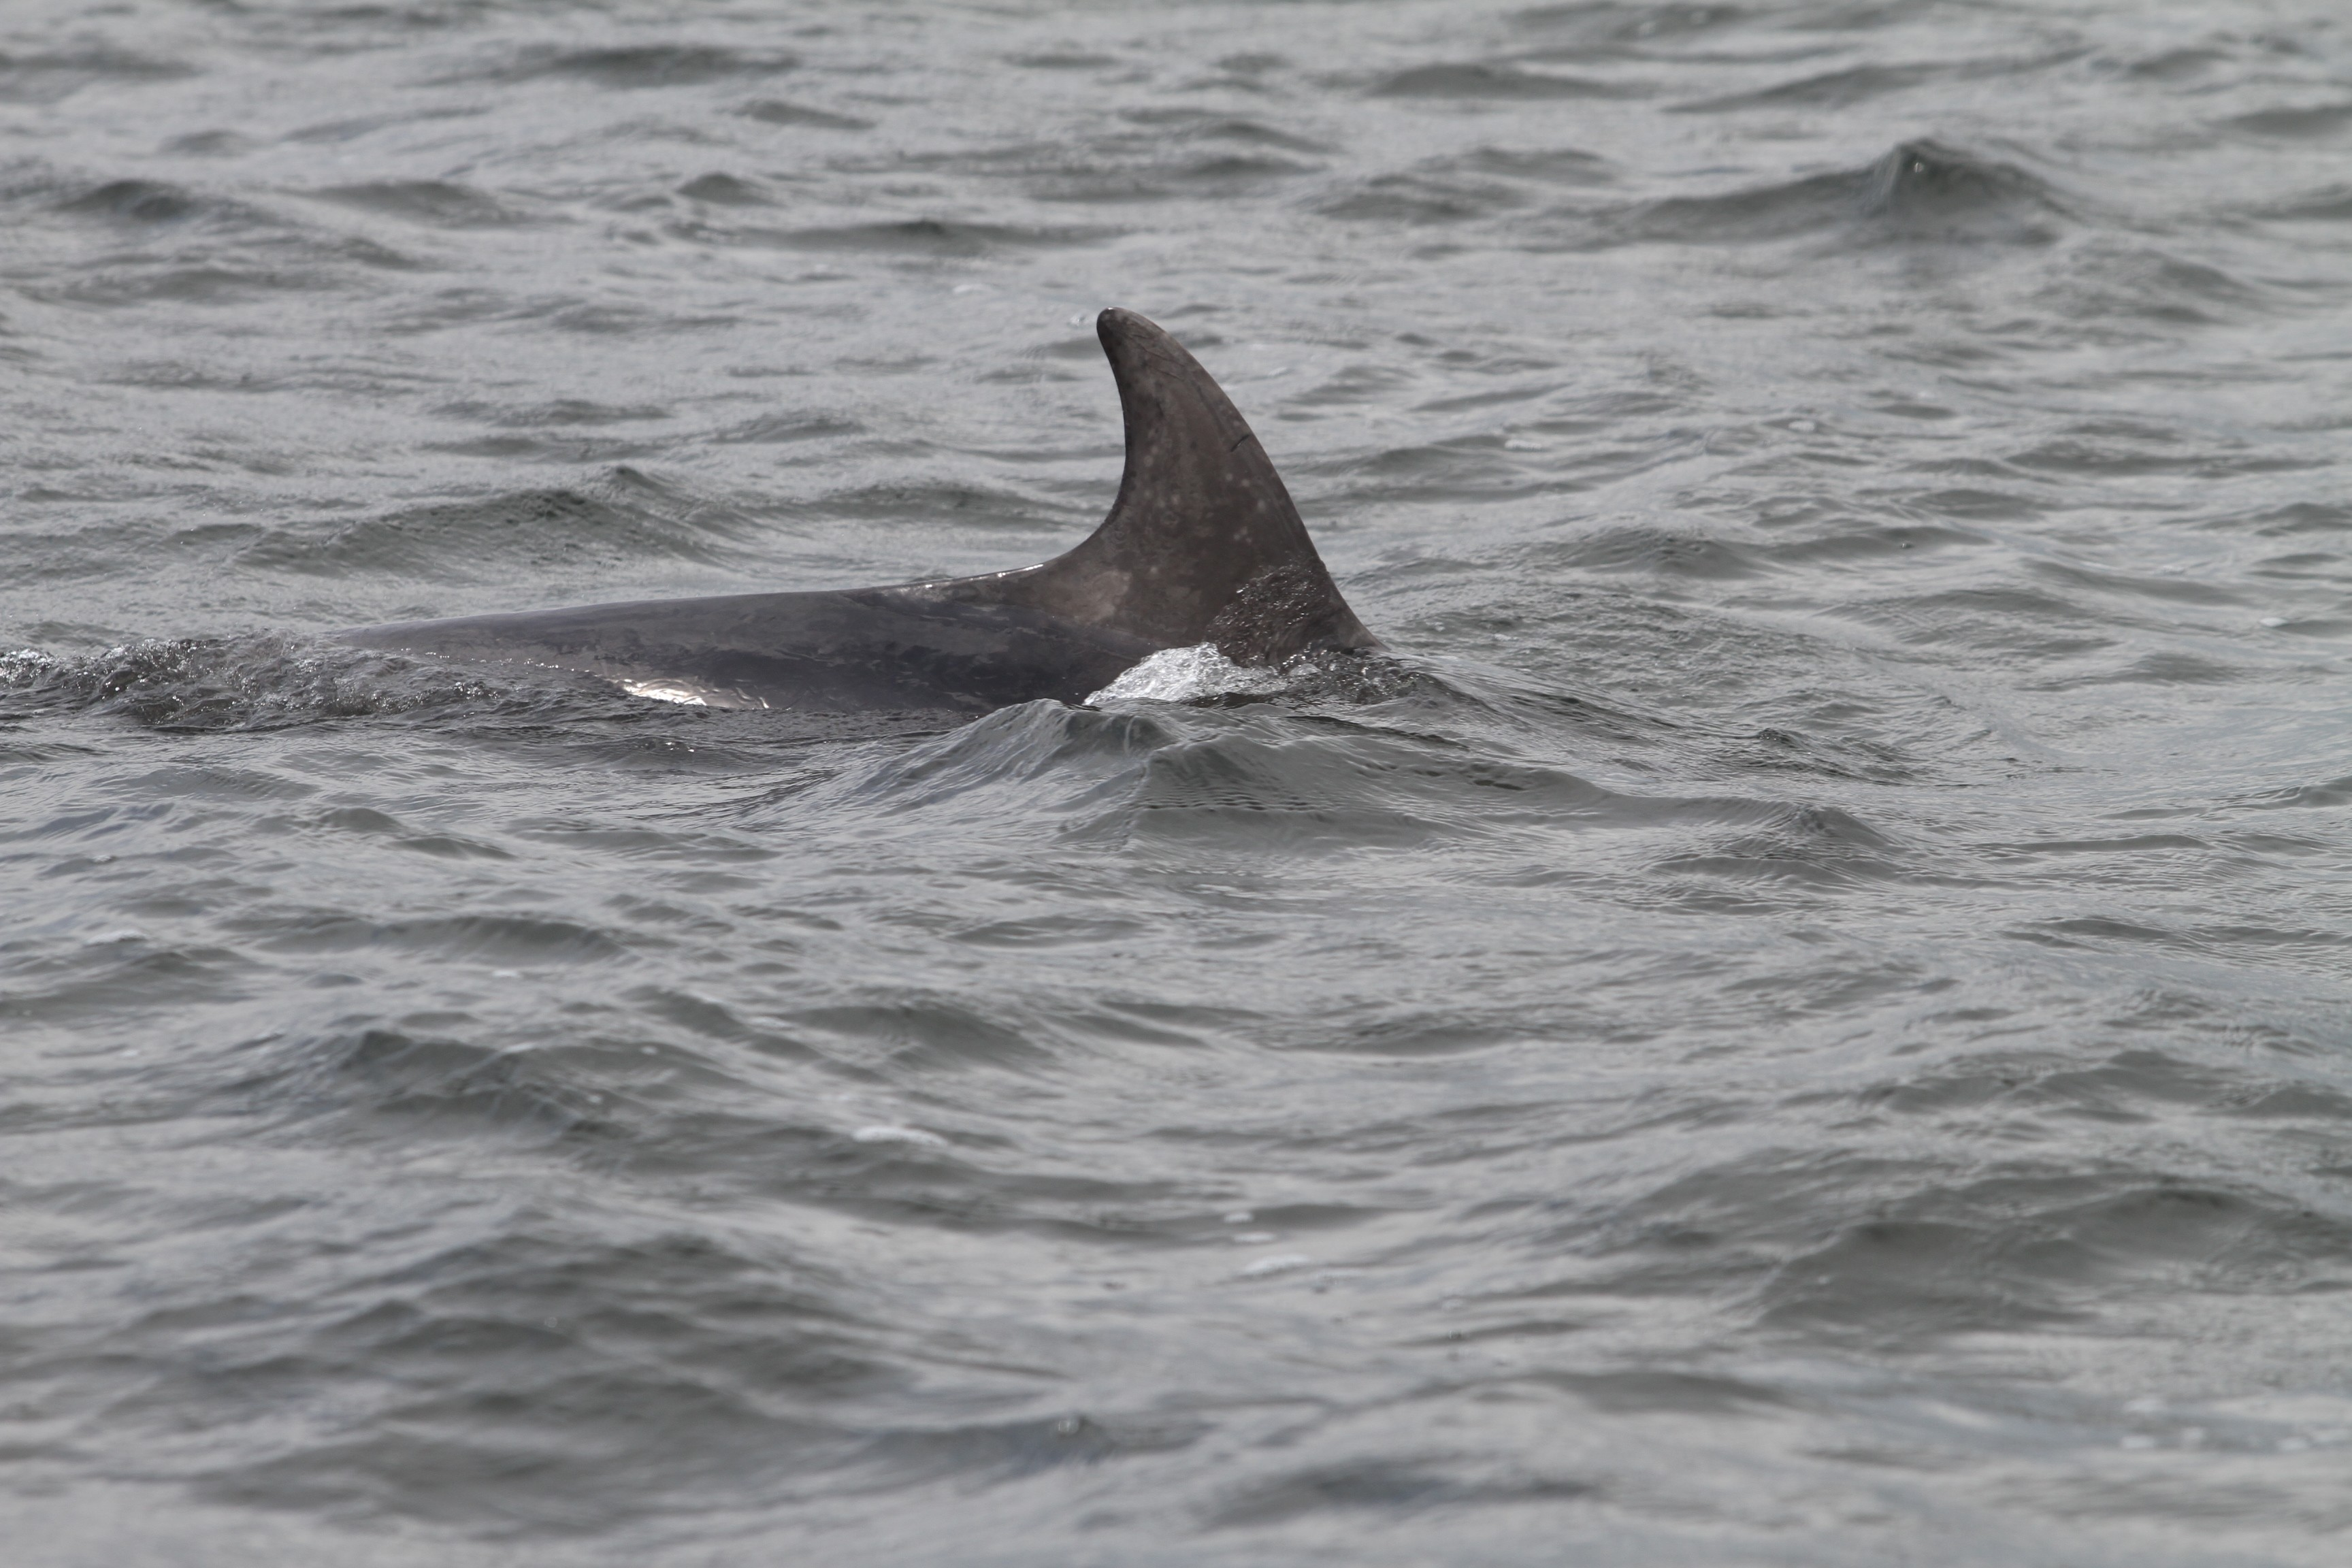
\includegraphics[width=0.8\textwidth]{example_train.jpg}
    \caption{Example image of a bottlenose dolphin}
    \label{fig:example_train}
\end{figure}

\begin{figure}
    \centering
    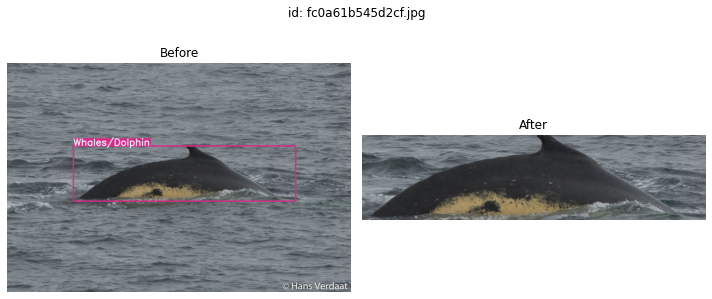
\includegraphics[width=0.8\textwidth]{image_cropping.png}
    \caption{Animal detection using YoloV5 model}
    \label{fig:image_cropping}
\end{figure}


The training images came in a variety of sizes. Figure \ref{fig:example_train} shows an example unprocessed image. Large amounts of each image are just of water which is irrelvant to the classification task. We are only interested in the parts of the 
images that contain the animals.

A solution to this issue was proposed within the discussions of the Kaggle competition \cite{cropped_dataset_kaggle}. YoloV5 was trained on a dataset of 1200 pictures of whale flukes and the corresponding location of points on the edge of the fluke for those pictures \cite{whale_fluke_dataset}. 
This was then assumed to generalise to finding the bounding box for any part of a whale or dolphin within the water. However, it is worth noting that finding the bounding box of any part of the animal is considered an Out of Distribution problem. From this technique a cropped dataset was created with all images having a dimension of 256 x 256. This is the dataset that was then used to train the whale 
and dolphin classifier.


\section {Image Transformation}

A custom PyTorch dataset class called \emph{WhaleDataset} was created for loading in the training images. One-hot encoding was used for the image lables, representing the individual ids provided.

The images were converted to RGB format as this was the compatible format for PyTorch. The images were then transformed using the TorchVision transforms package. The images were already all the same dimension from the preprocessing outlined in the previous section. 
The transformation involved converting the PIL image to a PyTorch tensor, scaling ther pixel values to the range [0,1] followed by normalizing the tensor by subtracting the mean and dividing by the standard deviation.

Scikit Learn's \emph{train\_test\_split} was used to divide the data into training and test datasets using an 80/20 split. A random state was specified for reproducability between training runs. Shuffling was enabled on the test set.


\section{Network Architecture}

\begin{figure}
    \centering
    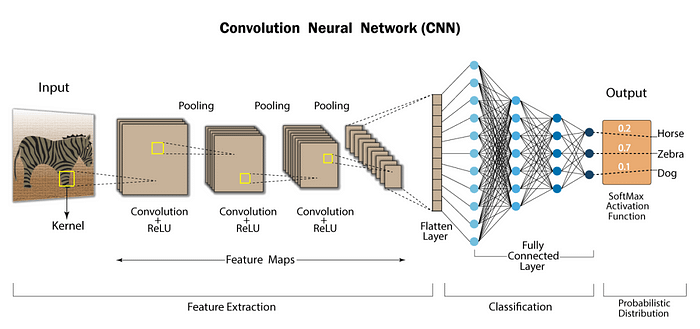
\includegraphics[width=0.8\textwidth]{cnn.png}
    \caption{Example of a CNN}
    \label{fig:network_architecture}
\end{figure}

A convolutional network architecture was selected for this problem. Three convolutional layers were selected for the network architecture so that increasingly more complex and 
abstract features could be extracted from the input image.

\begin{itemize}
    \item \verb|conv1|  takes the input image with 3 color channels (RGB) and applies 32 different 3x3 convolutional filters to extract low-level features like edges, corners, and simple patterns
    \item \verb|conv2| takes the output of the previous layer (32 feature maps) and applies 64 different 3x3 convolutional filters to detect slightly more complex patterns and features.
    \item \verb|conv3| takes the output of the previous layer (64 feature maps) and applies 128 different 3x3 convolutional filters to detect even more complex patterns and higher-level features that are useful for distinguishing between different classes.
\end{itemize}

After each convolutional layer, a ReLU activation function is applied to introduce non-linearity to the network

After the convolutional layers, there are two fully connected layers. The first fully connected layer takes the flattened output of the convolutional layers and applies a linear transformation, mapping to a fixed-sized vector of 512. This layer acts as a non-linear feature extractor, learning a higher-level representation of the convolutional features. A ReLU activation function is applied after this layer to introduce non-linearity.
The final fully connected layer applies a linear transformation, mapping the 512-dimensional vector to a vector of size equal to tthe number of unique individual\_ids in the training data.


\section{Model Training}

The Adam optimizer, a robust gradient-based optimization method, was chosen. Adam allows for faster convergence, compared to stochastic gradient descent, by adapting the learing rate during training \cite{kingma2017adam}

The PyTorch \emph{CrossEntropyLoss} criterion \cite{cross_entropy_loss} was used this was a multi-class classification problem. This criterion first applies a Softmax function on the logits, converting them into a propability distribution over the classes. Then the cross-entropy loss measures the performance of the model by comparing the predicted probability distribution with the true distribution (represented by the one-hot encoded target labels). It calculates the negative log-likelihood of the true class probabilities, penalizing the model more for being confident about the wrong predictions.

Despite the massive reduction in file size that came from using the cropped dataset instead of the original dataset, training times on the local machine were still prohibitively long. Therefore, training was done using AWS Sagemaker using a ml.p3.8xlarge GPU instance.

The hyperparameters under consideration were

\begin{itemize}
    \item \verb|Epochs|: Number of complete passes of the training dataset through the network
    \item \verb|Learning Rate|: The size of the step taken adjusting the model parameters during the optimization stage
    \item \verb|Batch Size|: The number of training examples passed through the network before backpropagation and optimization
\end{itemize}

An intial training run using a batch size of 32, a learning rate of 0.01 and training for 5 epochs gave a test accuracy of 0.87\%. Given the number of classes, this translates to the model predicting correctly 8 or 9 out of 1000 samples.
Increasing the learning rate had no impact on performance whilst reducing the learning rate reduced the performance. A smaller learning rate should lead to a higher accuracy \cite{smith2018dont} so this may be due to underfitting where the model parameters doesn't receive sufficient updates.


Reducing batch size made no material difference to performance. Smaller batch-size reduces the risk of overfitting however the model may already be well-regularized.

Training for additional epochs lead to a small improvement in accuracy. However, looking at Figure \ref{fig:training_loss}, the training loss was beginning to converge beyond the 5th epoch so continued training risked overfitting.

Dropout was added to the classifer architecture with a dropout rate of 0.2. Again this made no difference to performance so again overfitting is not the cause of poor performance.

A forth convolutional layer was then added to the network structure under the assumption a deeper network could capture more patterns within the images but also did not yield performance improvements. 

\begin{figure}[ht]
    \centering
    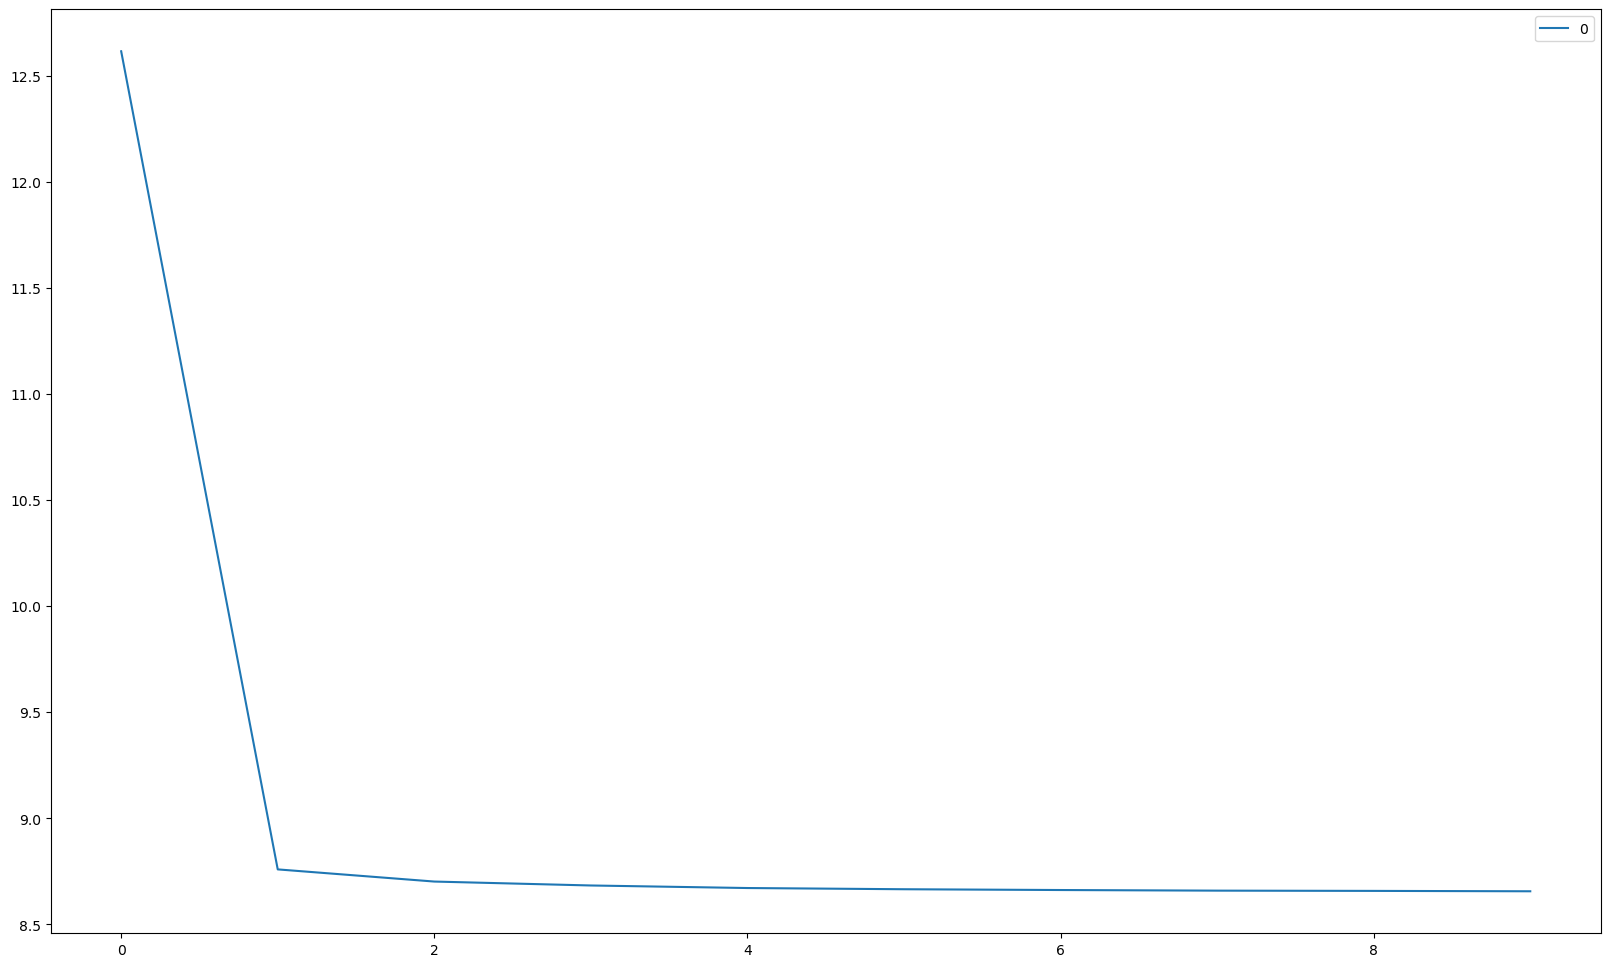
\includegraphics[width=0.5\textwidth]{train_loss.png}
    \caption{Training loss}
    \label{fig:training_loss}
\end{figure}

\begin{table}[ht]
\centering
\begin{tabularx}{\textwidth}{|X|X|X|X|X|X|}
\hline
\textbf{Epochs} & \textbf{Learning Rate} & \textbf{Batch Size} & \textbf{Loss} & \textbf{Accuracy} & \textbf{Notes} \\
\hline
5 & 0.01 & 32 & 10.6497 & 0.87\% & \\
\hline
5 & 0.1 & 32 & 10.7591 & 0.87\% &  \\
\hline
5 & 0.001 & 32 & 17.1580 & 0.72\% & \\
\hline
5 & 0.01 & 16 & 10.6052 & 0.87\% & \\
\hline
10 & 0.01 & 16 & 10.3002 & 0.86\% & \\
\hline
10 & 0.01 & 16 & 10.0023 & 0.86\% & Added Dropout \\
\hline
10 & 0.01 & 16 & 10.0001 & 0.86\% & Additional Conv2d layer \\



\hline
\end{tabularx}
\caption{Test Loss and Accuracy with different hyperparameter configurations}
\label{tab:example}
\end{table}

\section{Conclusions}

Performance achived by the model can be considered poor. This can be attributed to several factors

\begin{itemize}
    \item Differences between individuals with a species are very slight and can change over time
    \item Large class inbalance in the number of examples per species and per individual
    \item Computational limitations meant each model could only be trained for a few epochs
\end{itemize}

With additional time and computational resources, it is beleived performance gains could be made by first creating a model to classifiying the image for 
species before passing on species specific classifier that could then classify for the individual. The assumption being that a species specific model would
be easier to train to capture the nuances of each individual.


Additionally, it would be of interest to see if performance improvements could be made via contrast enhancement as an image preprocessing step. The animals were 
similar colors to the ocean so something that could emphasis the shape of the animal could assist the model.



\bibliographystyle{plain}
\bibliography{references}

\end{document}
